\documentclass[12pt]{beamer}
\usetheme{Pittsburgh}
\usepackage[T1,T2A]{fontenc}
\usepackage[utf8]{inputenc}
\usepackage[bulgarian]{babel}
%\usepackage{amsmath}
%\usepackage{amsfonts}
%\usepackage{amssymb}
\usepackage{graphicx}

%\usepackage{enumerate}
%\usepackage{soul}

\title{Информационна система на агенция за недвижими имоти}
\subtitle{Част I: Приложение на принципите за контекстуално проектиране}
\author{Екип $\pi \approx 3.1$}

%\setbeamercovered{transparent} 
\setbeamertemplate{navigation symbols}{} 
\date{} 

\begin{document}

\begin{frame}
\titlepage
\end{frame}

%\begin{frame}
%\tableofcontents
%\end{frame}

\begin{frame}[fragile]
\frametitle{Екип $\pi \approx 3.1$}
\begin{center}

\begin{tabular}{r|l}
%\hline
71469	& Георги Димов \\ %\hline
71473	& Цветан Цветанов \\ %\hline
71488	& Антон Дудов \\ %\hline
71490	& Венцислав Конов \\ %\hline
71492	& Александър Танков \\ %\hline
71508	& Красимир Тренчев \\ %\hline
71512	& Александър Велин \\ %\hline
71524	& Анджелика Туджарска \\ %\hline
71529	& Александър Бранев \\ %\hline
855240	& Мартин Стоев \\ %\hline
\end{tabular}

\end{center}
\end{frame}

\begin{frame}[fragile]
\frametitle{Обща представа за системата}
	\begin{itemize}
	\item Трябва да се проектира информационна система за стартираща агенция за недвижими имоти, която до момента не е използвала никакви системи и няма съществуващи към момента бизнес процеси. 
	\item Описаната тук система е според изискванията на собственика на агенцията.
	\end{itemize}
\end{frame}

\begin{frame}[fragile]
\frametitle{Обща представа за системата}
	\begin{itemize}
	\item Целта на информационната система е да осигури уеб интерфейс, чрез който брокерите могат да управляват своите обяви за недвижими имоти, а клиентите на агенцията (наематели и купувачи) да имат гъвкав и удобен интерфейс за търсене на обяви за имоти по различни критерии, както и да инициират комуникация с брокера.
	\item Връзката между собствениците на имоти и брокерите ще се осъществява извън рамките на системата.
	\item Всички счетоводни и финансови процеси в агенцията не са предмет на информационната система.
	\end{itemize}
\end{frame}

\begin{frame}[fragile]
\frametitle{Интервюта}
Бяха проведени две интервюта със собственика на агенцията Борислав Арнаудов:
	\begin{itemize}
		\item на 2016-03-18 от 16:00 до 17:30 в зала 01 на ФМИ
		\item на 2016-04-01 от 09:00 до 10:30 в САП България
	\end{itemize}
\end{frame}

\begin{frame}[fragile]
\frametitle{Flow models}
На базата на събраната информация бяха идентифицирани следните роли:
\begin{itemize}
	\item нерегистриран потребител;
	\item регистриран потребител;
	\item брокер;
	\item администратор;
	\item одитор.
\end{itemize}
За всяка роля беше проучен и описан съответстващият ѝ модел на дейностите.
\end{frame}

\begin{frame}[fragile]
\frametitle{Нерегистриран потребител}
		\begin{itemize}
		\item {Търсене на обяви}
		\item {Споделяне на обяви}
		\item {Връзка с брокер през контакт форма}
		\item {Използване на чат}
		\item {Регистрира се}
		\end{itemize}
\end{frame}

\begin{frame}[fragile]
\frametitle{Нерегистриран потребител}
	\begin{figure}[h]
	\centering
	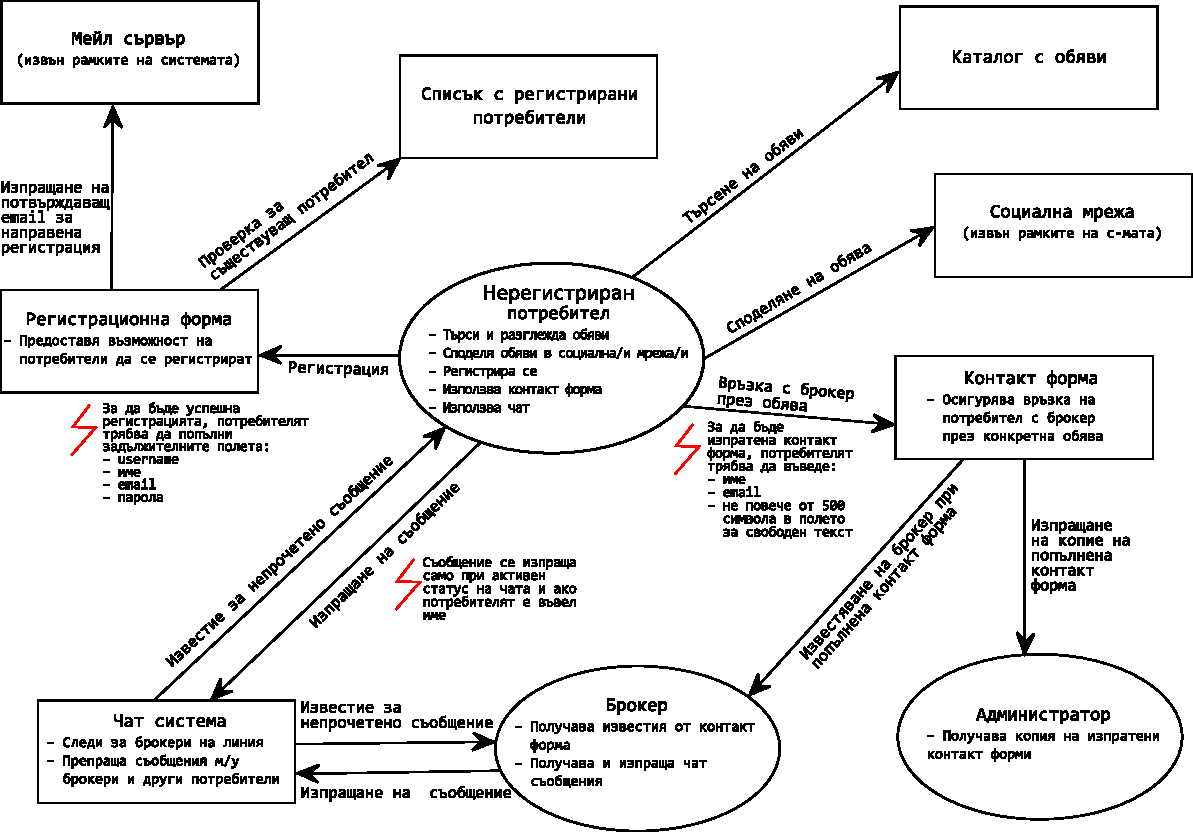
\includegraphics[scale=0.50]{flow-unregistered-user}
	\end{figure}
\end{frame}

\begin{frame}[fragile]
\frametitle{Регистриран потребител}
		\begin{itemize}
		\item същите възможности, които има и нерегистрираният потребител
		\item история на чат сесиите
		\item може да запазва обява към профила си
		\end{itemize}
\end{frame}

\begin{frame}[fragile]
\frametitle{Регистриран потребител}
	\begin{figure}[h]
	\centering
	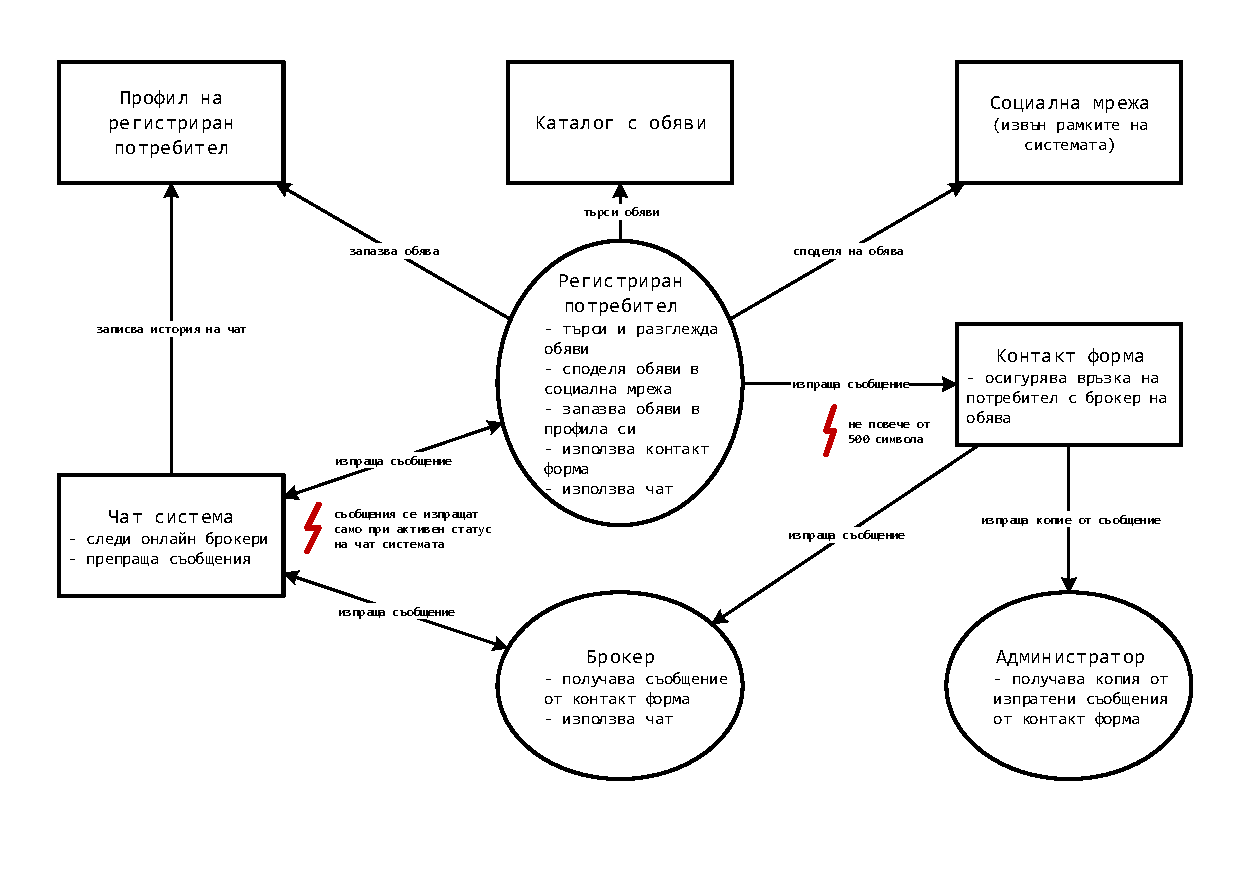
\includegraphics[scale=0.55]{a1-flow-reg}
	\end{figure}
\end{frame}

\begin{frame}[fragile]
\frametitle{Брокер}
		\begin{itemize}
		\item същите възможности, които има и регистрираният потребител
		\item създава и редактира обяви
		\item комуникира със собствениците извън системата
		\item получава съобщения през формата за контакти
		\end{itemize}
\end{frame}

\begin{frame}[fragile]
\frametitle{Брокер}
	\begin{figure}[h]
	\centering
	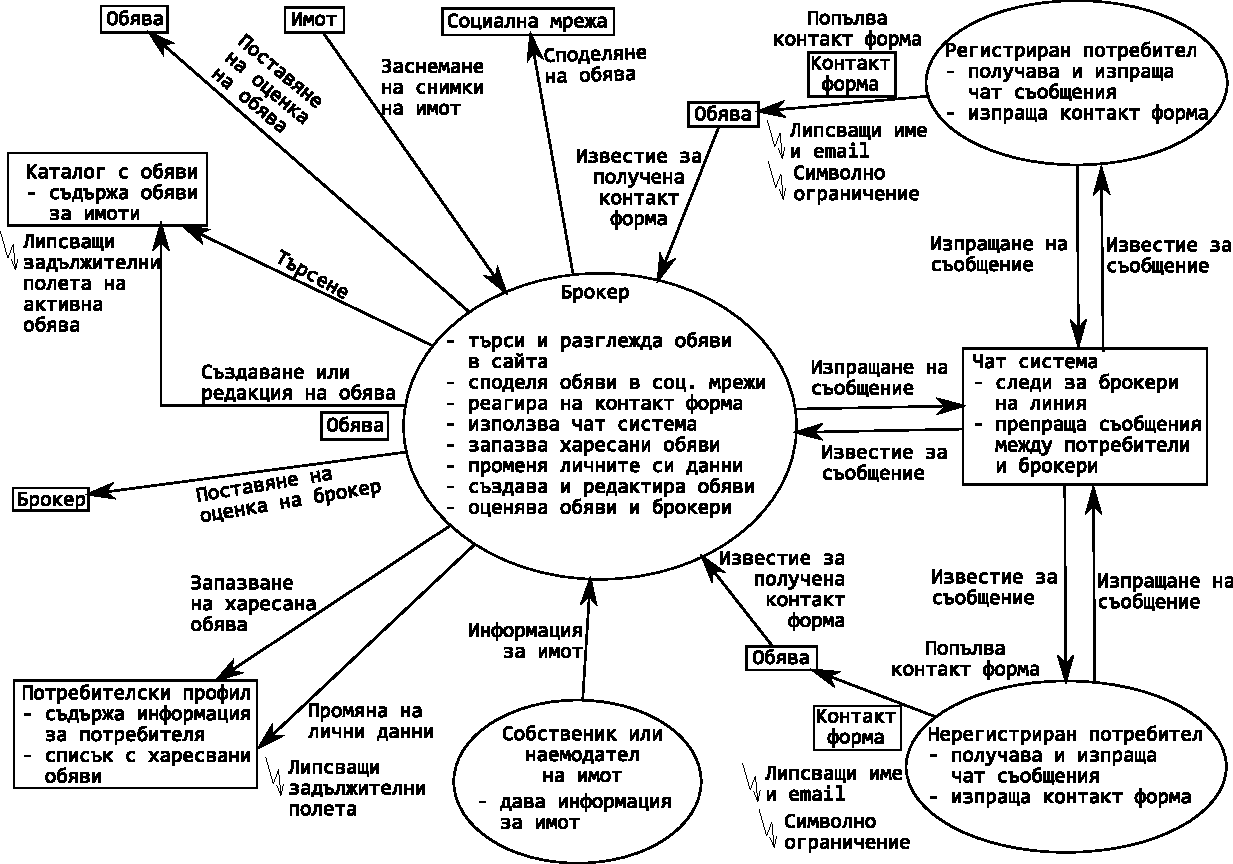
\includegraphics[scale=0.50]{flow-broker}
	\end{figure}
\end{frame}

\begin{frame}[fragile]
\frametitle{Администратор}
		\begin{itemize}
		\item вграден в системата акаунт
		\item същите възможности, които има и регистрираният потребител
		\item променя статуса на обяви - нормална/vip, публикувана/непубликувана
		\item изтрива обяви
		\item променя активния брокер за обява
		\item одобряване на заявки за брокер
		\item отнемане на статус ``брокер''
		\item копие от съобщения от контактната форма, препращане
		\end{itemize}
\end{frame}

\begin{frame}[fragile]
\frametitle{Администратор}
	\begin{figure}[h]
	\centering
	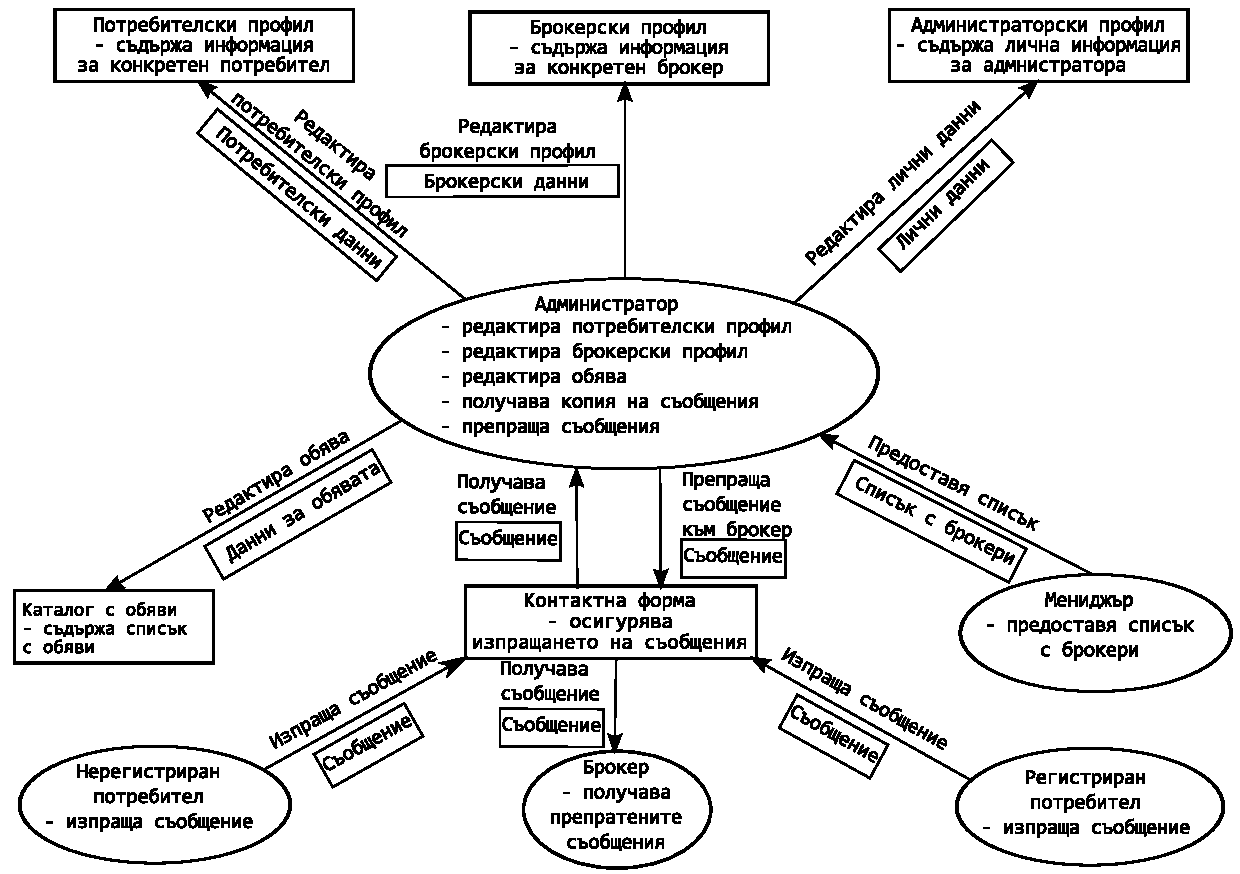
\includegraphics[scale=0.50]{flow-administrator}
	\end{figure}
\end{frame}

\begin{frame}[fragile]
\frametitle{Одитор}
		\begin{itemize}
		\item вграден в системата акаунт
		\item има права само да чете одит лога
		\item информация за настъпила промяна в системата
		\item правилата за допуск са извън обхвата на системата
		\end{itemize}
\end{frame}

\begin{frame}[fragile]
\frametitle{Одитор}
	\begin{figure}[h]
	\centering
	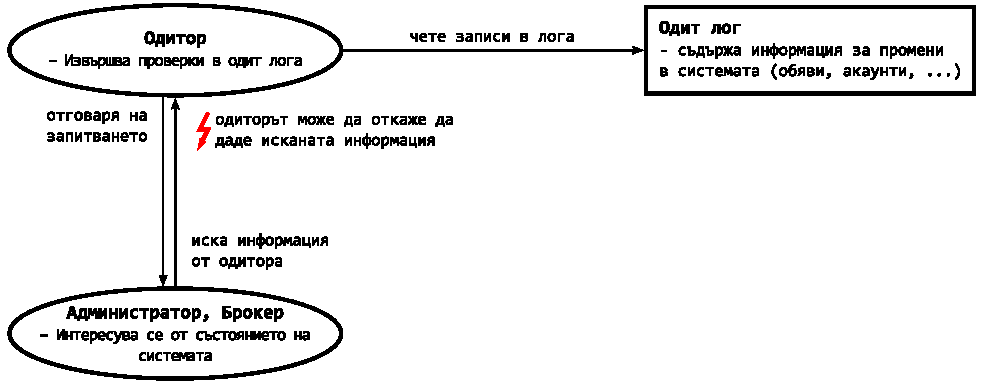
\includegraphics[scale=0.70]{flow-auditor-small}
	\end{figure}
\end{frame}

\begin{frame}[fragile]
\frametitle{Sequence models}
Моделирани последователности:
\begin{itemize}
	\item търсене на обява
	\item регистриране на потребител
	\item брокер добавя имот
\end{itemize}
\end{frame}

\begin{frame}[fragile]
\frametitle{Търсене на обява}
\begin{center}
\scalebox{0.5}{
  \begin{tabular}{ |p{7cm}|p{12cm}| }
    \hline
    \multicolumn{2}{|c|}{\textbf{Намерение}: Потребител желае да потърси обяви по даден критерий.} \\    \hline
    & \textbf{Тригер}: Потребител натиска бутон ``Търси''. \\    \hline
    \textbf{Намерение}: Да се намери обява в регион, удобен за потребителя. & Появява се списък с населени места, ако е на мобилно устройство, иначе се появява карта на страната. \\    \hline
    \textbf{Бележка}: Потребителят може да се върне назад за да поправи критерия. & \\    \hline
      & Потребителят се препраща към стъпка за избиране на район/квартал. \\    \hline
    \textbf{Намерение}: Да се намери обява в квартал/район, удобен за потребителя. & Появява се карта на текущо избраното населено място, от която потребителят може да избира квартал/район. Ако е на мобилно устройство се появява само списък. \\    \hline
    \textbf{Бележка}: Потребителят може да се върне назад за да поправи критерия. & \\    \hline
     & Потребителят се препраща към стъпка за избиране на характеристики на имота. \\    \hline
    \textbf{Намерение}: Да се избере имот, който спазва нужните на потребителя характеристики. & Появяват се полета с характеристики, от които потребителят може да избира. Валидно е да се избере повече от една характеристика. \\    \hline
    \textbf{Бележка}: Потребителят може да се върне назад за да поправи критерия. & \\    \hline
     & Предоставя се поле за търсене. \\    \hline
    \textbf{Намерение}: Филтриране на получените резултати чрез търсене в текстовите полета на обявите. & Предоставя се поле за търсене, където потребителят въвежда свободен текст. По този свободен текст се филтрират тези обяви, които го имат в полетата си. \\    \hline
    \textbf{Бележка}: Потребителят може да се върне назад за да поправи критерия. & \\    \hline
    \textbf{Намерение}: Уведомяване на потребителя за наличните обяви. & Повявява се списък с обявите спазващи горните четири критерия. \\    \hline
  \end{tabular}
  }
\end{center}

\end{frame}

\begin{frame}[fragile]
\frametitle{Регистриране на потребител}
\begin{center}
\scalebox{0.5}{
  \begin{tabular}{ |p{7cm}|p{12cm}| }
    \hline
    \multicolumn{2}{|c|}{\textbf{Намерение}: Нерегистриран потребител желае да се регистрира} \\
    \hline
    & \textbf{Тригер}: Потребил натиска бутон ``регистрация''. \\
    \hline
      \textbf{Намерение}: Потребителят попълва данните & Показва се форма за попълване на личните данни на потребителя. \\
    \hline
     & След попълването се изчаква потребителя за натискане на бутон ``регистрирай ме''. \\
    \hline
    \textbf{Намерение}: Проверка на данните, въведени от потребителя. & Потребителското име се проверява за уникалност. \\
    \hline
     & Паролите въведени от потребителя се проверяват спрямо критериите за сигурност. \\
    \hline
     & Проверка за валидност на email адреса. \\
    \hline
     & Името се проверява дали съдържа само букви. \\
    \hline
    \textbf{Бележка}: Потребителя се уведомява за грешка ако такава съществува.  & \\
    \hline
      & Потребителя се препраща към полето при което има грешка, ако са повече от една се препраща към първото поле. \\
    \hline
    \textbf{Намерение}: Добавяне на номер на телефон и снимка. & Ако потребителят е осигурил номер на телефон и снимка, те се добавят в потребителския акаунт.  \\
    \hline
    \textbf{Намерение}:  Верификация на вече създадения потребителски акаунт. & Изпраща се email до адреса, въведен от потребителя.  \\
    \hline
     & След изпращането се изчаква за потвърждаване от страна на потребителя. \\
    \hline
    \textbf{Намерение}: Съхранение на паролата на потребителя. & Изчаква се обработката и запазването на потребителската парола от страна на външната система\\
    \hline
    \textbf{Намерение}: Уведомяване на потребителя за успешно регистриране. & Потребителят бива препратен към страницата за вход. \\
    \hline
  \end{tabular}
  }
\end{center}
\end{frame}

\begin{frame}[fragile]
\frametitle{Брокер добавя имот}
\begin{center}
\scalebox{0.6}{
  \begin{tabular}{ |p{6cm}|p{10cm}| }
    \hline
    \multicolumn{2}{|c|}{\textbf{Намерение}: Брокер желае да създаде обява} \\
    \hline
    	& \textbf{Тригер}: Брокерът натиска бутон ``Създаване на обява''. \\
    \hline
    	\textbf{Намерение}: Брокерът попълва данните & След попълването на полетата на обявата се изчаква натискане на бутон ``Създай обявата''  \\  
	\hline
    	\textbf{Намерение}: Проверка на данните въведени от брокера & Проверява се обявата има ли снимка \\
    \hline
    	& Проверява се обявата има ли скица \\
    \hline
    	& Проверява се обявата има ли цена \\
    \hline
    	& Проверява се обявата има ли обявено място на имота \\
    \hline
        \textbf{Бележка}: Брокера се уведомява за грешка ако не е попълнено някое задължително поле & \\
    \hline     
    	& Брокера се препраща към полето, което не е попълнено. Ако са повече от едно, се препраща към първото. \\
    \hline
    	\textbf{Намерение}: Уведомяване за успешно създаване на обява & \\
    \hline
  \end{tabular}
  }
\end{center}
\end{frame}

\begin{frame}[fragile]
\frametitle{Artifact models}
Моделирани артефакти:
\begin{itemize}
	\item данни за определена обява - адрес, цена, характеристични полета, снимки и т.н.
	\item списък с всички брокери на агенцията (на хартия)
\end{itemize}
\end{frame}

\begin{frame}[fragile]
\frametitle{Данни на обява}
		\begin{itemize}
		\item Жизненият статус на обявата може да бъде Активен или Неактивен, като съответно се вижда или не от потребителите.
		\item Преференциалният статус може да бъде VIP обява или Обикновенна обява, като VIP обявите се показват първи при търсене.
		\item Вход, етаж и апартамент са видими само за ролите администратор и брокер.
		\item GPS координати - точна локация, изобразява се чрез Google Maps.
		\item Снимките и скиците - поне една снимка и една скица, като общо да са най-много 20. Всяка с размер до 1 MB.
		\item Свободният текст да е най-много 5000 знака.
		\end{itemize}
\end{frame}

\begin{frame}[fragile]
\frametitle{Данни на обява}
	\begin{figure}[h]
	\centering
	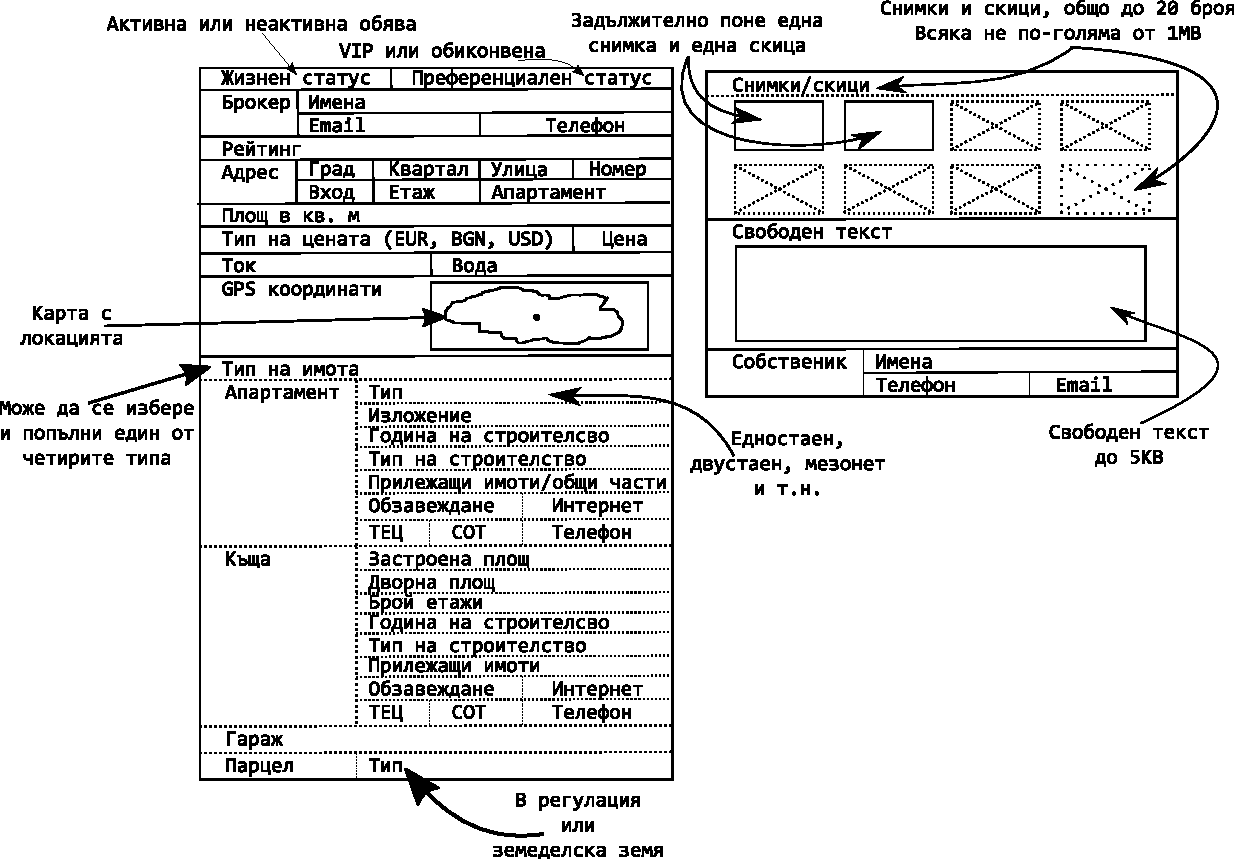
\includegraphics[scale=0.50]{art-offer}
	\end{figure}
\end{frame}

\begin{frame}[fragile]
\frametitle{Списък с брокери}
	\begin{itemize}
	\item списък (на хартия) с всички брокери на агенцията
	\item мениджърът го предоставя на администратора
	\item заглавна част
	\item номер на записа
	\item три имена на одобрените брокери
	\item email адрес на одобрения брокер.
	\item дата на наемане
	\item заключителна част
	\end{itemize}		
\end{frame}

\begin{frame}[fragile]
\frametitle{Списък с брокери}
Име и email адрес са полетата, по които администраторът идентифицира наетите от фирмата брокери. Ако акаунт, поискал повишение в брокер, не притежава характеристики, идентични с описаните в документа, то администраторът отхвърля искането. Ако характеристиките съвпадат, администраторът повишава акаунта в брокер. При нужда от добавяне на описание на нови брокери, артефактът минава в притежание на мениджъра, докато бъде попълнен, след което се връща отново при администратора. 
\end{frame}

\begin{frame}[fragile]
\frametitle{Списък с брокери}
	\begin{figure}[h]
	\centering
	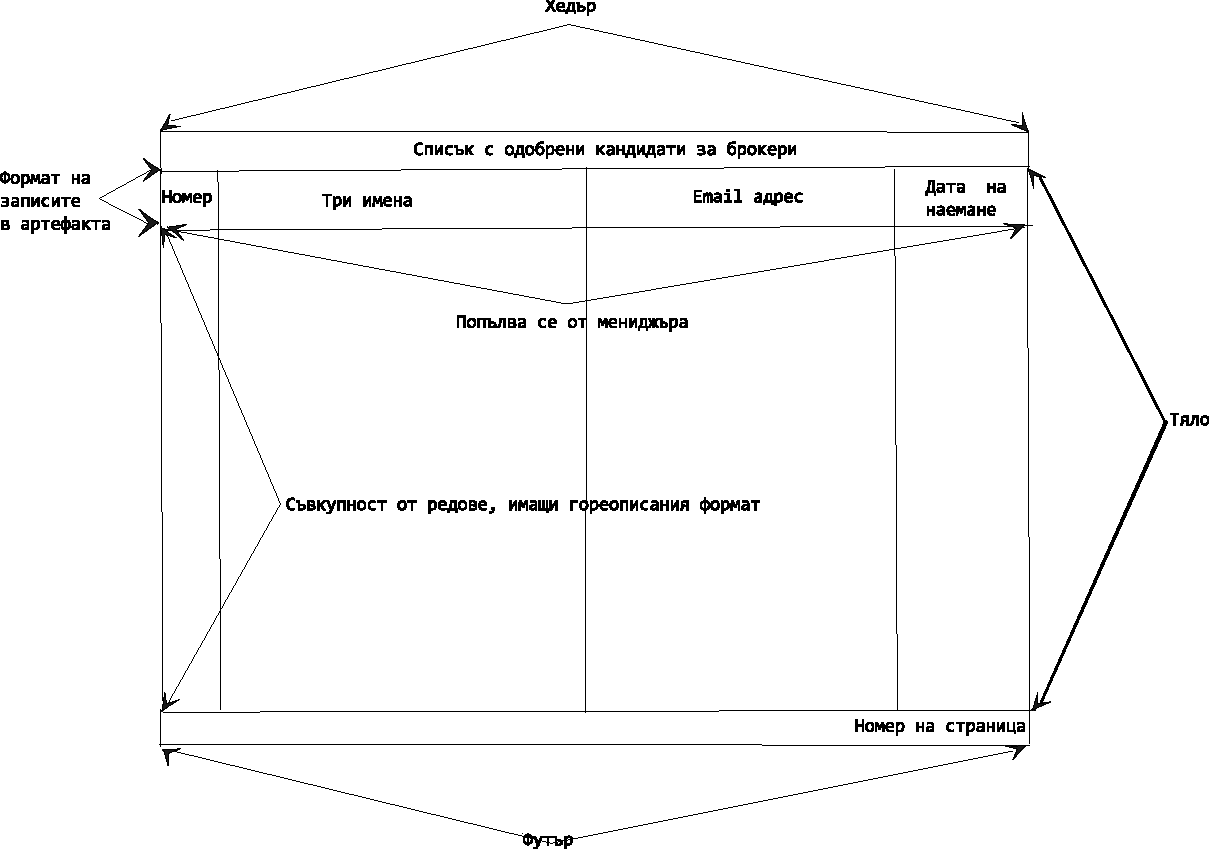
\includegraphics[scale=0.52]{art-textFile}
	\end{figure}
\end{frame}


\end{document}
